%%%%%%%%%%%%%%%%%%%%%%%%%%%%%%%%%%%%%%%%%%%%%%%%%%%%%%%%%%%%%%%%%%%
%                                                                 %
%  GEANT manual in LaTeX form                              %
%                                                                 %
%  Michel Goossens (for translation into LaTeX)                   %
%  Version 1.00                                                   %
%  Last Mod. Jan 24 1991  1300   MG + IB                          %
%                                                                 %
%%%%%%%%%%%%%%%%%%%%%%%%%%%%%%%%%%%%%%%%%%%%%%%%%%%%%%%%%%%%%%%%%%%
\Origin{R.Brun,F.Bruyant,A.McPherson}
\Submitted{01.11.83}                     \Revised{18.11.93}
\Version{Geant 3.16}\Routid{GEOM199}
\Makehead{The volume data structure -- JVOLUM}

\section{The data structure {\tt JVOLUM} and {\tt JGPAR}}

The meaning of the variables in the data structure {\tt JVOLUM} shown
in fig. \ref{fg:geom199-1}
is the following:

\begin{DLtt}{MMMMMMMM}
\item[ISEARC] search flag {\tt [GEOM400], [GEOM410]}:
\begin{DLtt}{MMMM}
\item[$=$0] volume positioning order or ordering by \Rind{GSNEXT}/\Rind{GSNEAR};
\item[$<$0] binary search as defined by \Rind{GSORD};
\item[$>$0] user ordering \Rind{GSUNEA}/\Rind{GUNEAR};
\end{DLtt}
\item[ISHAPE] system shape number (see {\tt [GEOM050]};
\item[NIN] number of volumes contained in the mother volume --
if negative the volume is divided;
\item[NMED] medium number for the volume;
\item[NPAR] number of shape parameters;
\item[NATT] number of attributes;
\item[PAR] array of shape parameters;
\item[IAT] array of attributes;
\item[IAXIS] direction of the division (see {\tt [GEOM130]});
\item[IVO] system volume number;
\item[NDIV] number of divisions ({\tt -NDVMX}, if computed dynamically,
see {\tt [GEOM140]});
\item[C0] coordinate value at which the division starts;
\item[STEP] coordinate step for the division;
\item[NR] user copy number;
\item[IROT] rotation matrix number defining the orientation of the volume
with respect to the mother reference system;
\item[X,Y,Z] position of the volume with respect to the mother reference
system;
\item[KONLY] {\tt ONLY/MANY} flag, see {\tt [GEOM110]} for more information;
\end{DLtt}
 
\begin{figure}[hbt]
     \centering
     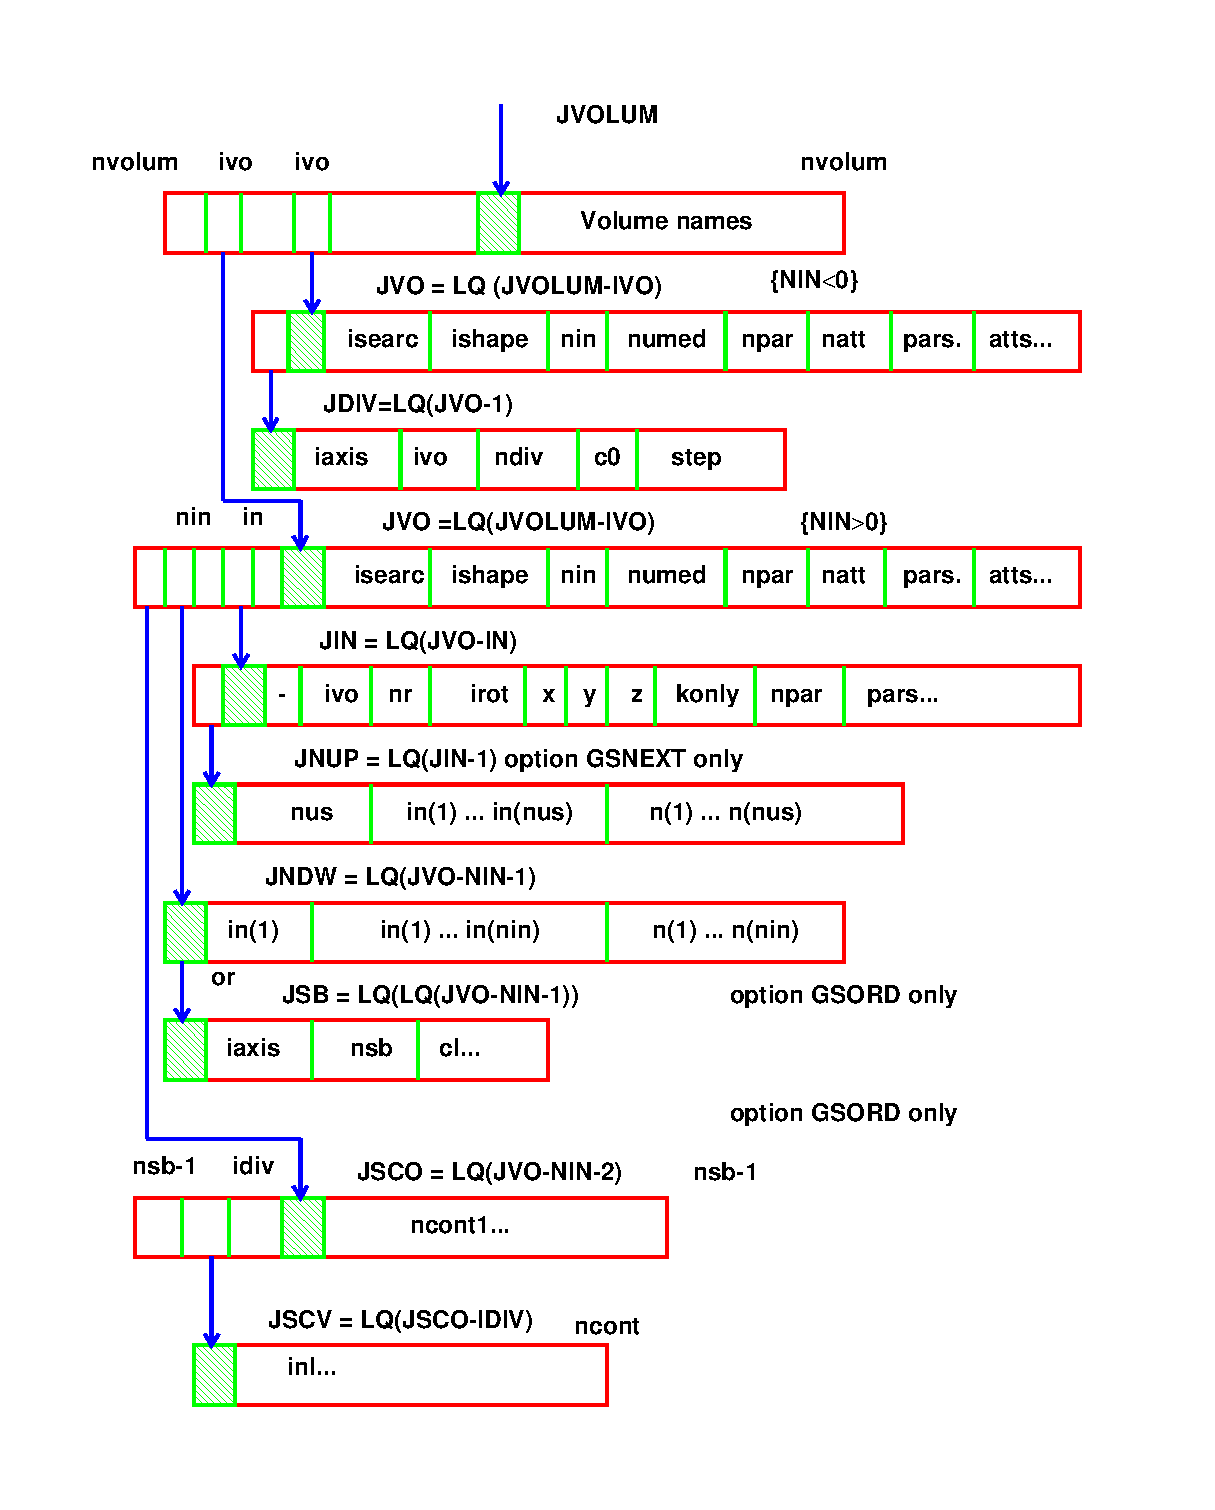
\epsfig{file=eps/geom199-1.eps,width=14cm}
     \caption{Example of geometrical tree structure}
     \label{fg:geom199-1}
\end{figure}
